% !TEX root = mfe.tex

\section{Definition of multi-stranded DNA systems and basic lemmas}\label{sec:mfe}

Intuitively, a single DNA strand $s$ is a sequence of nucleotide bases connected by covalent bonds which together make up the backbone of $s$, with the left end of the sequence corresponding to the $5'$ end of $s$ and the right end corresponding to the $3'$ end. When drawing $s$ we label  the $3'$ end with an arrow which also shows the strand directionality, see \cref{fig:sec struct}. Hydrogen bonds can form between Watson-Crick base pairs, namely C–G and A–T.

Formally, A DNA strand $s$ is a word over the alphabet of DNA {\em bases} $\{\mathrm{A},\mathrm{T},\mathrm{G},\mathrm{C}\}$, indexed from 1 to $|s|$, where $|s|$ denotes the length of $s$.
A base pair is a tuple $(i, j)$ such that $i<j$. 
For any $c$ strands, we will assign to each of them a unique distinct identifier in $\{1, . . . ,c\}$~\cite{dirks2007thermodynamic}. Each base is specified by a strand identifier and a position on that strand, $i_s$ denotes the base of index $i$ of strand $s$.

\subsection{Connected unpseudoknotted secondary structures and  polymer graphs}

\begin{Definition}[Secondary structure $S$]
	For any set of $c$ DNA strands, a secondary structure $S$ is a set of base pairs such that each base appears in at most one pair, i.e.~if $(i_n, j_m)\in S$ and $(k_q, l_r)\in S$ then $i_n,j_m,k_q,l_r$ are all distinct.
\end{Definition}
The {\em graph representation of a  secondary structure} $S$
is the graph $G=(V,E)$, where $V$ is the set of bases of each strand $s \in \{1, . . . ,c\}$, and $E = E_v \cup E_b$, where $E_v$ is the set of \emph{covalent backbone bonds} connecting base $i_n$ with base $(i+1)_n$ for all bases $i = 1,2, ..., |n|-1$ on all strands $n \in \{1, . . . ,c\}$, and $E_b = S$ is the set of base pairs in $S$. $E_v$ and $E_b$ are disjoint.

The set of circular permutations, $\Pi$, of $c$ strands has $(c-1)!$ distinct circular permutations~\cite{brualdi1977introductory} (e.g., for the three strands $\{A, B, C\}$, $\Pi = \{A B C, ACB\}$), 
e.g., the orderings $ABC$, $BCA$, and $CAB$ are the same on a circle. 
Next, we define a  polymer graph for each $\pi$, see also  \cref{fig:sec struct}.

\begin{Definition}[Polymer graph]
	For any secondary structure $S$, and any ordering $\pi$ of its $c$ strands, the polymer graph representation of $S$,  denoted  \PolySpi, is a graph representation of $S$, embedded in the unit disk from $\mathbb{R}^2$, where the $c$ strands are placed in succession from their $5'$ to $3'$ ends around the circumference of the circle, and the bases, $V$, are spaced evenly around the circle circumference, each element of $E_v$ is represented by an arc on the circumference between covalently-bonded bases, and each element of $E_b$ is represented by a chord between two different bases. 
\end{Definition}

\begin{Definition}[Unpseudoknotted secondary structure]
	A secondary structure $S$ is unpseudoknotted if there exists at least one circular permutation $\pi \in \Pi$ such that $\PolySpi$ is planar, otherwise $S$ is pseudoknotted. 
	An example is shown in \cref{fig:sec struct}.
\end{Definition} 


\begin{remark}
	In the rest of the paper we use $N$ to denote the total number of bases of a secondary structure $S$.
	A secondary structure $S$ is connected if the graph representation of $S$ is a connected graph. In this work, we are only interested in connected unpseudoknotted secondary structures.
\end{remark}

\begin{figure}[t]
	\centering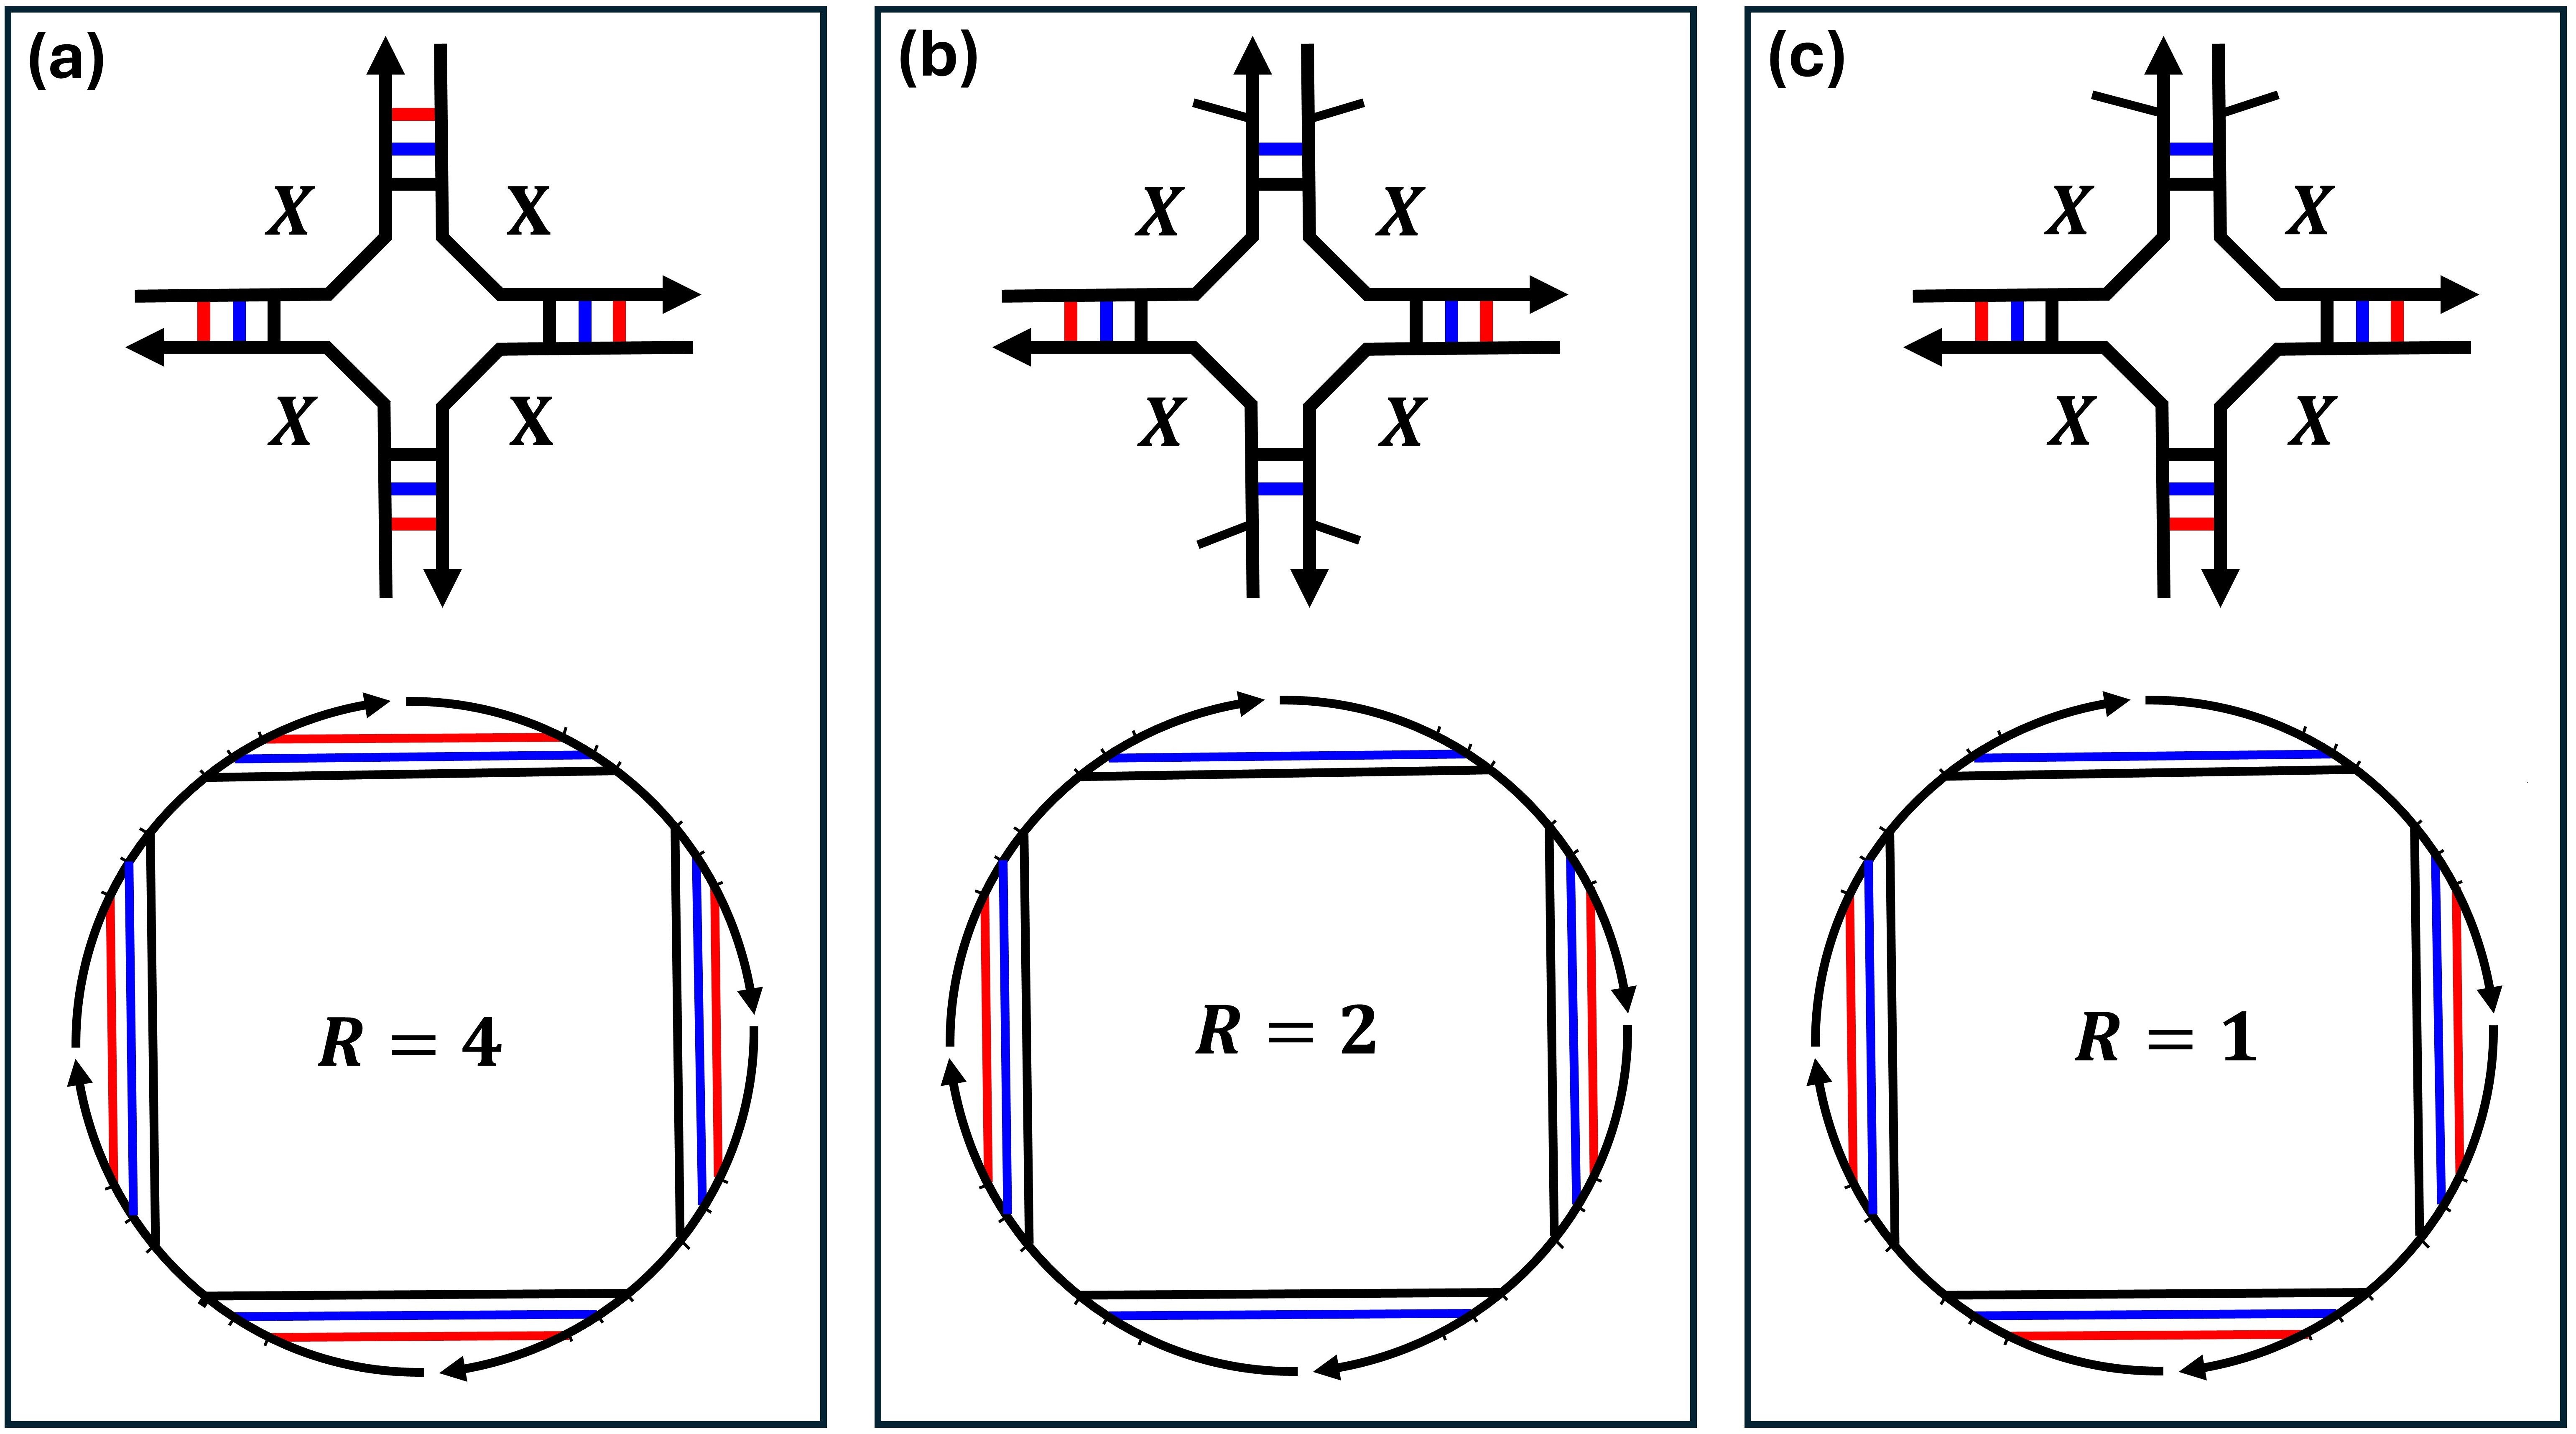
\includegraphics[width=0.7\textwidth]{figures/sym.jpg}
	
	\caption{Three secondary structures  with their associated polymer graphs. In each case, there is a single complex with four identical (indistinguishable) strands of  strands of type $X$, but with different symmetry degree $R$. 
		(a)~Symmetry degree $R$ = 4 (rotation by $90^{\circ}$  gives the same secondary structure). 
		(b)~Symmetry degree  $R$ = 2 (rotation by $180^{\circ}$  gives the same secondary structure). 
		(c)~Symmetry degree  $R$ = 1 (asymmetric secondary structure).
	}\label{fig:sym}
\end{figure}

\subsection{Free energy of a secondary structure}
Any connected unpseudoknotted secondary structure $S$ can be decomposed into different loop types~\cite{tinoco,santa,mathews1999expanded}: namely hairpin loops, interior loops, exterior loops, stacks, bulges, and multiloops as shown in \cref{fig:sec struct}. 
As usual, let  $k_B$ be Boltzmann's constant and $T$ is the temperature in Kelvin (also a constant).\footnote{All results hold if we assume these are typical values from physics, or just 1 in appropriate units.} 
The free energy of $S$ is defined as the sum of three terms:\footnote{Throughout this paper $\log n = \log_\mathrm{e} n$.}
\begin{equation}\label{eq:DGss}
	\Delta G(S) =  \sum_{l\in S} \Delta G(l) + (c-1)\Delta G^{\textrm{assoc}} + k_\mathrm{B} T \log R.
\end{equation}  
\begin{itemize}
	\item the first is itself the sum of the (well-defined, empirically-obtained) free energies $\Delta G(l)$ of $S$'s constituent loops~\cite{dirks2007thermodynamic}, where each loop energy is defined with respect to the free energy of the unpaired reference state.
	\item $\Delta G^{\textrm{assoc}} $ is the entropic association~\cite{dirks2007thermodynamic} penalty applied for each of the $c-1$ strands added to the first strand to form a complex of $c$ strands.
	\item $R$ is the rotational symmetry of the secondary structure $S$,  illustrated in \cref{fig:sym}, and to be formally defined  in \cref{sec:sym}.  In particular, since favourable free energies are usually negative, the term  $k_\mathrm{B} T \log R \geq 0$ corresponds to the reduction in the entropic contribution of $S$, as any secondary structure with an $R$-fold rotational symmetry has a corresponding $R$-fold reduction in its distinguishable conformational space~\cite{dirks2007thermodynamic} as shown in \cref{fig:sym}.\footnote{This is perhaps counter-intuitive. In a follow-up expanded version of this paper we will give a full statistical mechanics explanation, which treats the symmetry penalty to offset the fact that non-symmetrical structures are undercounted.} Dynamic programming algorithms to date for mulit-stranded MFE ignored this term for reasons we outline in \cref{sec:sym}.
\end{itemize}



For $c$ strands, we let $\Omega$ be the set  (usually called the {\em ensemble}) of all  connected unpseudoknotted secondary structures. 
For any circular permutation $\pi \in \Pi$ of the $c$ strands, let $\Omega(\pi) \subseteq \Omega$ be the subset of $\Omega$ such that each connected unpseudoknotted secondary structure $S\in \Omega(\pi)$ is representable as a crossing-free polymer graph with circular permutation $\pi$. 
%\dw{: more precisely, $\pi$ is the ordering such that $\PolySpi$  has no crossings}.

\begin{remark}[$S$, or $\PolySpi$]\label{rm:PolySpi}
	Dirks et al.~\cite{dirks2007thermodynamic} showed, in their representation theorem (Theorem 2.1), that the sets $\Omega(\pi)$, for all $\pi \in \Pi$, form a partitioning of $\Omega$, which means that every connected unpseudoknotted secondary structure belongs to exactly one $\Omega(\pi)$ for some $\pi \in \Pi$. 
	Hence to avoid the cumbersome phrase 
	{\em $c$-strand connected unpseudoknotted secondary structure $S$ with strand ordering $\pi$ and polymer graph $\PolySpi$}
	we simply write $S$, or $\PolySpi$.
\end{remark}



Predicting the minimum free energy means finding a minimum over the ensemble $\Omega$. 
The known strategy is to deal with each partition $\Omega(\pi)$ separately,  
then finding their minimum:  
\begin{equation}\label{eq:MFE}
	\textrm{MFE} = \min_{S \in \Omega} \Delta G(S)  =\min\limits_{\pi \in \Pi} \left\{ \min_{S \in \Omega(\pi)} \Delta G(S) \right\}  
\end{equation}

\subsection{Definition of multi-stranded rotational symmetry} \label{sec:sym}

Here, we formalise rotational symmetry. 
In the previous section we assigned each one of the $c$ strands a unique identifier, dealing with them as distinct strands even if two or more have the same sequence. 
But in most experimental settings, strands with the same sequences are \emph{indistinguishable}   in the sense that they behave identically with respect to relevant measurable quantities~\cite{dirks2007thermodynamic}. 
Mathematically, we say that {\em two strands are  indistinguishable} if they have the same sequence. 
Also, two \emph{secondary structures are indistinguishable} if there exists a permutation of the implied unique strand ordering (\cref{rm:PolySpi}), 
that maps indistinguishable strands onto each other while preserving all base pairs, otherwise, the two structures are distinct~\cite{dirks2007thermodynamic}.


For any $c$ strands, not necessarily distinct, they consist of $k \leq c$ \emph{strand types}, usually denoted by uppercase English letters $X,Y,\ldots$\footnote{In contrast with some of the literature. we exclude using $\{\mathrm{A},\mathrm{T},\mathrm{G},\mathrm{C}\}$ for strand types; to avoid any confusion between strand and base types.}
A {\em multi-stranded DNA system} 
$M = \{(t_1,n_1),(t_2,n_2), ..,(t_k,n_k)\}$,  
is a \emph{multiset} of $k$ strand types $t_1,  ..., t_k$ with repetition numbers 
$n_1,  ..., n_k \in \mathbb{N}$ such that $n_1+ ...+n_k = c$.\footnote{It is known~\cite{sawada2003fast} how to efficiently reduce the circular permutation space by getting rid of  circular permutations that are redundant due to indistinguishable strands, which is important to consider when computing the  partition function but needed for MFE.} 
For such a multiset $M$
we can think of each circular permutation $\pi$  as a string over strand types such that each strand type $t_i$ appears exactly $n_i$ times (e.g., $M = \{(X,6),(Z,3)\}$ one valid $\pi$ is $\pi = XZXXZXXZX$). 



\begin{Definition}[Symmetry degree of a permutation] \label{def:sym}
	For any circular permutation $\pi$, we say $n \in \mathbb{N}$ is a symmetry degree of $\pi$ if $\pi = y^n$ for some $y$, a prefix of $\pi$. 
\end{Definition}

\noindent For example, $\{1,2,4\}$ are the symmetry degrees of $\pi = XZXZXZXZ$ since $\pi = (XZXZXZXZ)^1 = (XZXZ)^2 = (XZ)^4$.

For any circular permutation $\pi$, 
its maximum symmetry degree is denoted $v(\pi)$, and the corresponding repeating prefix $x$, such that $x^{v(\pi)} = \pi$, is the \emph{fundamental component} of $\pi$. 
It can be seen that $x$ is the smallest prefix that repeats over $\pi$. 
Indeed, $v(\pi)$ is the number of cyclic permutations that map each strand to a strand of the same type. 
Any repeating prefix of $\pi$ must be a multiple of its fundamental component, as proven in \cref{lem:factors} in \cref{sec:lemmasApp}.


\begin{remark}[Notation: $X_m^n$]
	For any circular permutation $\pi$, 
	its \emph{augmented version}  gives the full ordering information for each fundamental component. 
	For example, 
	if $\pi = XYXZ \, XYXZ$, then its fundamental component is $XYXZ$ and its augmented version is 
	$ X_1^1 Y_1^1 X_2^1 Z_1^1  \; X_1^2 Y_1^2 X_2^2 Z_1^2$, such that  $X_m^n$, means the $m$th strand of type $X$ in the $n$th fundamental component of $\pi$.   
\end{remark}

We can visualize any ordering $\pi$ by representing it as a \emph{regular $v(\pi)$-gon} with each of its $v(\pi)$ vertices   representing a fundamental component. %, evenly placed on a circle. 
Let $\rho = (1 \ 2 \ 3 \ ... \ v(\pi))$\footnote{Here we use algebraic cycle notation.  
	The order of $\rho$, denoted by $o(\rho)$, is the length of $\rho$ which is $v(\pi)$.} and consider the cyclic group\footnote{$G^\pi$ is isomorphic to $C_{v(\pi)}$, cyclic group of order $v(\pi)$.} $G^\pi$ generated by $\rho$. Intuitively, $G^\pi$ is the group of the all $v(\pi)$ rotational motions in plane of the regular $v(\pi)$-gon that give the same $v(\pi)$-gon. 
We can represent  $G^\pi$ as follows:  $G^\pi = \{\rho^0, \rho^1 ...,\rho^{v(\pi)-1}\}$, where $\rho^i$ represents rotation of the regular $v(\pi)$-gon by the angle of  
$i \times {\frac{360^{\circ}}{v(\pi)}}$, 
where  $|G^\pi| = v(\pi)$.


Now, we are ready to define the rotational symmetry of a secondary structure and a strand ordering $\pi$, intuitively, the number of rotations of its polymer graph that give the same polymer graph, as shown in \cref{fig:sym}.


\begin{Definition}[$R$-fold rotational symmetric structure]  \label{def:sym}
	A connected unpseudoknotted secondary structure $S$ and strand ordering $\pi$ 
	(and thus polymer graph $\PolySpi$) 
	is $R$-fold rotational symmetric, 
	or simply rotationally symmetric, 
	then for any base pair $(i,j)$ in the polymer graph $\PolySpi$
	the rotation of that base pair by multiples of $(360^\circ/R)$ is also in $\PolySpi$. 
	More formally:   
	$(i_{X_k^l},j_{Y_m^n}) \in \PolySpi$,   
	iff 
	$(i_{X_k^{a(l)}}, j_{Y_m^{a(n)}}) \in \PolySpi$ for all $a \in H \! \leq \! G^\pi$, where $H$ is the largest subgroup\footnote{$H \leq G$, notationally means $H$ is a subgroup of $G$. Every subgroup of cyclic group is also cyclic.} satisfying the condition, and if $|H| = R$.  
\end{Definition}


\begin{remark}
	In Def. \ref{def:sym},	we restricted $H$ to be the {\em largest} subgroup so as to be aligned with the entropic reduction penalty due to symmetry that appears in \cref{eq:DGss}, even if  from a geometric perspective any $R$-fold rotational symmetric secondary structure should be also $R'$-fold rotational symmetric if $R'$ divides $R$. 
\end{remark}


\section{A polynomial upper bound on a class of rotationally symmetric secondary structures}\label{sec:ub}


\begin{remark}\label{rm:noNicks}
	In this section, we assume a global indexing of all bases from $1$ to $N$, and use square brackets, $[i, i+1]$, to  denote the covalent bond connecting bases $i$ and $i +1$, given that both belong to the same strand. This notation also helps to differentiate covalent bonds $[i, i+1]$ from base pair $(j,k)$ (hydrogen bonds)  notation. 
\end{remark}

\begin{Definition}[$R$-symmetric backbone cut generated by a covalent bond]\label{def:cut}
	For  a connected unpseudoknotted secondary structure $S$ and strand ordering $\pi$, the {\em $R$-symmetric backbone cut generated by the covalent bond} $b=[i_{A_m^n}, (i+1)_{A_m^n}]$ is $\mathcal{C}_R^b = \{ [i_{A_m^{a(n)}}, ({i+1})_{A_{m}^{a(n)}}]: \textrm{ for all } a \in H \!\!\leq \!\! \!\ G^\pi \textrm{ such that } |H| = R \}$. We call $b$ a {\em symmetric backbone cut generator}. An example is shown in \cref{fig:sand}.
\end{Definition}


Only one covalent bond is needed to generate its corresponding $R$-symmetric backbone cut. Also, note that this definition excludes any cut through nicks by \cref{rm:noNicks}. The next lemma shows that the number of unique symmetric backbone cuts is linear in $N$.

\subsection{Linear upper bound on number of unique symmetric backbone cuts}

\begin{lemma}[Upper bound on unique symmetric backbone cuts]\label{lem:ub}
	For any connected unpseudoknotted secondary structure $S$ of $c=\mathcal{O}(1)$ strands with $N$ total bases, with a specific strand ordering $\pi$, the number of  unique symmetric backbone cuts is $\frac{N-c}{v(\pi)} \left[ \sigma(v(\pi))-v(\pi) \right] = \mathcal{O}(N)$, where $\sigma(v(\pi))$ is sum of divisors of $v(\pi)$. 
\end{lemma}

\begin{proof}\textcolor{red}{TOPROVE 0}\end{proof}


If $S$ is a connected unpseudoknotted secondary structure with ordering $\pi$, you can go from any base $i$ to $j$ in two different paths around the circumference of $\PolySpi$ (clockwise or anticlockwise). We define the \emph{length} function $l[i,j]$ to be the length of the shorter path, including both $i$ and $j$ as follows: 
\begin{equation}
	l[i,j] = \min \{|i-j|+1,N-|i-j|+1\}
\end{equation} 

Also,  $\llbracket i,j \rrbracket$  is used to denote that shorter {\em segment} of length $l[i,j]$, where the direction from base $i$ to base $j$ is the same as the system strands' direction.    

\subsection{How to slice a pizza (secondary structure)}

{\bf We} want to slice any $R$-fold rotational symmetric secondary structure $S$, {\bf like pizza}, to the centre of its $\PolySpi$, without intersecting any of its base pairs. First, we formalise (\cref{def:admissible}) a special type of backbone cut, called an \emph{admissible  $R$-symmetric backbone cut}. Then, we will prove (\cref{lem:cutexist}) its existence for $S$. 

\begin{Definition}[Admissible $R$-symmetric backbone cut] \label{def:admissible}
	For any connected unpseudoknotted secondary structure $S$ with strand ordering $\pi$, the {\em $R$-symmetric backbone cut} $\mathcal{C}_R^b$ generated by $b$ is {\em admissible}, 
	if for all covalent bonds $x \in \mathcal{C}_R^b$,  
	$x$ is not ``enclosed'' by any base pair $(i,j) \in \PolySpi$, more formally:  $x \nsubseteq \llbracket i,j \rrbracket$.   An example is shown in \cref{fig:sand}.
\end{Definition}


\begin{restatable}{lemma}{cutexist} 
	\label{lem:cutexist}
	For any $R$-fold rotationally symmetric secondary structure $S$, there exists at least one admissible $R$-symmetric backbone cut of $S$.
\end{restatable}
\begin{proof}\textcolor{red}{TOPROVE 1}\end{proof}

Note that any $R$-fold rotationally symmetric secondary structure $S$ can have more than one admissible R-symmetric cut. Before defining what we mean by a pizza slice (formally, symmetric slice in \cref{def:symmetric slice}),  the following lemma is used to  ensure such a slice is  connected.

\begin{restatable}[Pizza slicing lemma] {lemma}{connected} 
	\label{lem:connected}
	For any $R\geq 2$ and any $R$-fold rotational symmetric secondary structure $S$, let $G$ be the graph obtained from $\PolySpi$ by removing the covalent bonds of admissible $R$-symmetric backbone cut $\mathcal{C}_R^b$ generated by any covalent bond $b$, such that $G=(V(\PolySpi), E(\PolySpi)\setminus\mathcal{C}_R^b)$, then $G$ is disconnected and consists exactly of $R$ connected isomorphic components.
\end{restatable}  




\begin{proof}\textcolor{red}{TOPROVE 2}\end{proof}

\begin{Definition}[Symmetric slice]\label{def:symmetric slice}
	From the construction in \cref{lem:connected}, each of the $R$ 
	isomorphic subgraphs (components) in $ \mathcal{G}$ is called a {\em symmetric slice} of $\PolySpi$,  denoted  by $\rhd^{S}$. Also, the loop free energy of a symmetric slice is: 
	\begin{equation}
		\Delta G(\rhd^{S}) = \sum_{l\in \rhd^{S}} \Delta G(l)
	\end{equation}
\end{Definition}

For any $R$-fold symmetric secondary structure $S$, the following lemma shows the existence of a unique loop in the center of $\PolySpi$  surrounded by the outer base pairs of its symmetric slices. We call it the {\em central loop} of $S$, and denote it by $\bigcirc^S$. This central loop plays a crucial role in validating our slicing and swapping strategy  (\cref{lem:sand,lem:sand2}) and determining the exact upper bound (\cref{lem:polyub}) of symmetric secondary structures need to be backtracked.  


\begin{restatable}{lemma}{centralloop} 
	\label{lem:centralloop}
	For any $R$-fold symmetric secondary structure $S$, there exists a single loop, that we call the central loop $\bigcirc^S$, that is not contained in any of the $R$ symmetric slices. 
	If $R>2$ then $\bigcirc^S$ is a multiloop, if $R=2$ then $\bigcirc^S$ is either a multiloop, stack, or an internal loop.   
\end{restatable}
\begin{proof}\textcolor{red}{TOPROVE 3}\end{proof}


Because of the crucial importance of multiloops for our strategy, we highlight the multiloop energy model that is used in the standard dynamic programming algorithms. The free energy of a multiloop has the following linear form~\cite{dirks2007thermodynamic}:
\begin{equation} \label{eq:multi}
	\Delta G^ \textrm{multi}  = \Delta G_\textrm{init}^\textrm{multi} + b \Delta G_\textrm{bp}^\textrm{multi} + n\Delta G_\textrm{nt}^\textrm{multi}.
\end{equation}
Where, $\Delta G_\textrm{init}^\textrm{multi}$ is called the penalty for   formation of the multiloop, $\Delta G_\textrm{bp}^\textrm{multi}$ is called the penalty for each of its $b$ base pairs that border the interior of the multiloop, and $\Delta G_\textrm{nt}^\textrm{multi}$ is called the penalty for each of the $n$ free bases inside the multiloop. For any $R$-fold symmetric secondary structure~$S$, 
$b \Delta G_\textrm{bp}^\textrm{multi}$ and $n\Delta G_\textrm{nt}^\textrm{multi}$ are shared equally between the $R$ symmetric slices of $\PolySpi$, hence $R$ divides both $b$ and $n$. So, we denote  $\Delta G^ \textrm{multi}  = \Delta G_\textrm{init}^\textrm{multi} + R(\Delta G_{\rhd^{S}}^\textrm{multi})$, where $\Delta G_{\rhd^{S}}^\textrm{multi}$ is the energy contribution of each symmetric slice of $\PolySpi$ to the multiloop free energy, such that $\Delta G_{\rhd^{S}}^\textrm{multi} = \frac{b}{R} \Delta G_\textrm{bp}^\textrm{multi} + \frac{n}{R} \Delta G_\textrm{nt}^\textrm{multi}$.

\begin{note}
	For any connected unpseudoknotted secondary structure $S$ of $c$ strands, we use $\overline{\Delta G}(S)$ to denote the \snMFE of $S$, in other words $\overline{\Delta G}(S) = \sum_{l\in S} \Delta G(l)
	+  (c-1)\Delta G^{\textrm{assoc}}$. It is clear that $\overline{\Delta G}(S) \leq \Delta G(S)$, as the symmetry correction $k_\mathrm{B} T \log R \geq 0$. 
\end{note}


\begin{figure}[t]
	\centering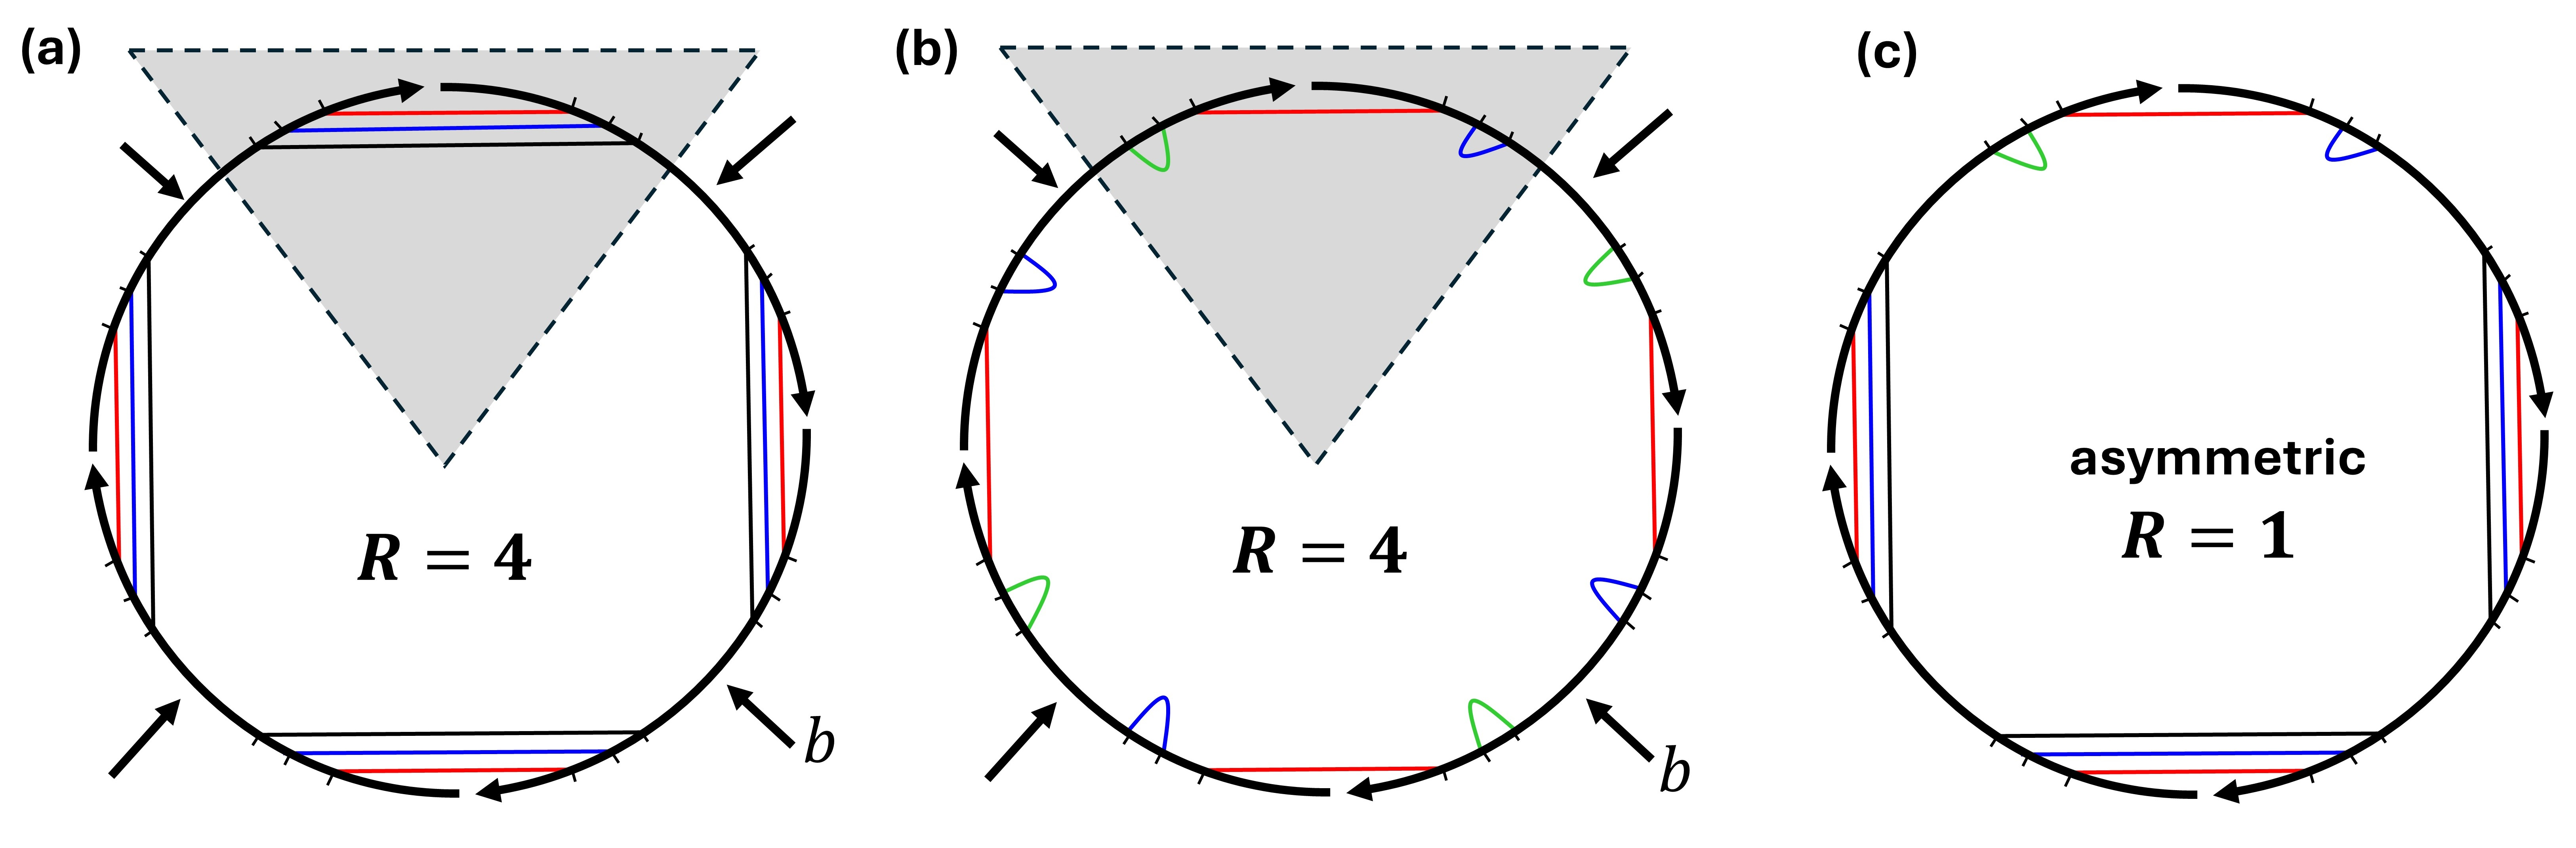
\includegraphics[width=0.7\textwidth]{figures/sand.jpg}
	\caption{Slicing and swapping strategy for constructing new asymmetric structure by combining two symmetric structures with the same symmetric backbone cut. 
		(a)~4-fold symmetric secondary structure $S_i$, with admissible $4$-symmetric backbone cut $\mathcal{C}_R^b$.
		Black arrows: indicate the four covalent bonds forming $\mathcal{C}_R^b$ generated by the covalent bond $b$. 
		(b)~4-fold symmetric secondary structure $S_j$, sharing the same cut $\mathcal{C}_R^b$ as $S_i$.
		Black arrows: indicate the four covalent bonds forming $\mathcal{C}_R^b$. 
		(c)~Asymmetric secondary structure $S_k$ that is constructed by replacing the grey shaded `slice' from $S_i$ by its corresponding slice from $S_j$, using the proof of  \cref{lem:sand}. 
	}\label{fig:sand}
\end{figure}



Intuitively, the following lemma lets us take two symmetric pizzas with the same admissible symmetric cut for which we merely now their \snMFE (we don't know their true MFE), and swap a slice from one into the other to get a new asymmetric pizza whose true MFE lies between their {\snMFE}s. The key intuition is that we transforming symmetric secondary structures into an  asymmetric one. 

\begin{lemma}\label{lem:sand}[Free-energy sandwich theorem for two $R$-fold rotational symmetric  structures]
	For any two distinct $(R \geq 3)$-fold rotationally symmetric secondary structures, $S_i$ and $S_j$, of $c$ strands, such that $R \geq 3$ and $\DGnosym(S_i) \leq \DGnosym(S_j)$ and $S_i$ and $S_j$ have the same R-admissible backbone cut $\mathcal{C}_R^b$, then there exists at least one asymmetric secondary structure $S_k$, such that $\DGnosym(S_i) \leq \Delta G(S_k) \leq \DGnosym(S_j)$.  Furthermore, the statement holds if $R=2$ and at least one of the central loops  $\bigcirc^{S_i},  \bigcirc^{S_j}$  is a multiloop. 
\end{lemma}

\begin{proof}\textcolor{red}{TOPROVE 4}\end{proof}

\cref{lem:sand} states that, if two symmetric secondary structures, having the same admissible R-symmetric backbone cut, belong to the same energy level based on \symnMFE algorithm, ignoring symmetry entropic correction, this implies the existence of at least one asymmetric secondary structure that actually belong to the same energy level because symmetry  correction for asymmetric structures is zero. If the two secondary structures belong to two different energy levels, then there exist at least one asymmetric secondary structure that actually belong to an energy level strictly lies between the other two energy levels.


\paragraph{Intuition for the case of $R=2$ and the central loop is not a multiloop.} 
When $R=2$, and the central loop is not a multiloop, the proof of \cref{lem:sand} breaks.   
From \cref{lem:centralloop}, when $R=2$ the central loop is either a multiloop, internal loop or stack loop. 
The multiloop case has been handled already (\cref{lem:sand}), and the stack loop case can be subsumed into the  internal loop case, since stacks are considered a special type of internal loop in the standard energy model~\cite{dirks2007thermodynamic}. 
Instead of depending on having the same admissible 2-symmetric backbone cut, we depend on sharing the same central internal loop itself, this more restricted hypothesis   implies having the same admissible 2-symmetric backbone cut too, allowing us to prove \cref{lem:sand2} using a similar strategy to  \cref{lem:sand}.  


\begin{lemma}\label{lem:sand2}[Free-energy sandwich theorem for two $2$-fold rotational symmetric structures]
	For any two distinct  $2$-fold rotationally symmetric secondary structures, $S_i$ and $S_j$, of $c$ strands, such that $\DGnosym(S_i) \leq \DGnosym(S_j)$ and both have the same central internal loop $\bigcirc^{S_i} = \bigcirc^{S_j}$, then there exists at least one asymmetric secondary structure $S_k$, such that $\DGnosym(S_i) \leq \Delta G(S_k) \leq \DGnosym(S_j)$.  
\end{lemma}
\begin{proof}\textcolor{red}{TOPROVE 5}\end{proof}

We now have two sandwich theorems that we can use to construct an asymmetric structure: \cref{lem:sand,lem:sand2}. In \cref{sec:BT} we give a backtracking algorithm to search for suitable $S_i$ and $S_j$, with the goal of  applying either one of these two sandwich theorems to $S_i$ and $S_j$. 
To get an overall polynomial bound for the backtracking algorithm, we wish to bound, given $S_i$, how many secondary structures to scan before finding a suitable $S_j$.    
\cref{lem:ub} gives this upper bound on this number  when applying \cref{lem:sand}. 
Next, \cref{lem:ub2} gives this upper bound  when applying  \cref{lem:sand2}. 

Unfortunately, the bound in \cref{lem:ub2} is larger than \cref{lem:ub}, since the energy model is more complex for internal loops than multiloops~\cite{dirks2003partition}. 

\begin{lemma}[Upper bound on number of  central internal loops]\label{lem:ub2}
	For any set of $c$ strands with specific ordering $\pi$, for any set $\mathcal{T}$ of $2$-fold rotational symmetric secondary structures $(R=2)$, 
	such that each has a distinct internal central loop, the  cardinality of $\mathcal{T}$, $ |\mathcal{T}| \leq \sum_{s\in y} (\lVert \baseA \rVert_s \lVert \baseT \rVert_s+ \lVert \baseG \rVert_s \lVert \baseC \rVert_s ) \leq N^2/16$, 
	where $y$ is a fundamental component of $\pi$, such that $\pi = y^2$, and $\parallel\! \! B \!\! \parallel_s$  
	denotes the number of bases in strand $s$ of type $B$ for all $B\in\{\mathrm{A},\mathrm{T},\mathrm{G},\mathrm{C}\}$.
\end{lemma} 

\begin{proof}\textcolor{red}{TOPROVE 6}\end{proof}









\subsection{Polynomial upper bound on number of symmetric secondary structures (for future backtracking)}
\begin{lemma}\label{lem:polyub}
	
	Given an ordering $\pi$ of $c$ strands, 
	for any set $\mathcal{T}$ of distinct symmetric secondary structures such that 
	\begin{enumerate}
		\item  for any two $(R>2)$-fold symmetric secondary structures $S_i, S_j \in \mathcal{T}$, where $S_i$ and $S_j$ have different admissible R-symmetric backbone cuts (we mean all possible cuts are different), 	
		and 
		\item 
		for any two 2-fold symmetric secondary structures $S_i, S_j \in \mathcal{T}$, where $S_i$ and $S_j$ have different admissible R-symmetric backbone cuts (all possible cuts are different)
		or  different central internal loops, 
	\end{enumerate}
	then $|\mathcal{T}| \leq \mathcal{U}$, where $\mathcal{U} =  \frac{N-c}{v(\pi)} \left[ \sigma(v(\pi))-v(\pi) \right] + \frac{N^2}{16} = \mathcal{O}(N^2)$. 
\end{lemma}

\begin{proof}\textcolor{red}{TOPROVE 7}\end{proof}

The (bad) quadratic bound in \cref{lem:ub2} is not that frequent: 
In particular, that bound only appears when $R=2$ and the central loop is an internal loop for both symmetric secondary structures (since $R=2$ this implies that the repetition number for every strand type is {\em even}, which in practice, say, for random or typical systems, may not be frequent).   
In particular the following lemma gives a {\em linear} bound when the repetition number of at least one strand type is odd. 


\begin{lemma} \label{lem:even}
	For any $R$-fold rotationally symmetric  secondary structure $S$, with ordering $\pi$, such that $R$ is even, then the repetition number of each strand type must be even. Hence for any system of $c$ strands ($k$ strand types) such that the repetition number of some strand type is odd, then $\mathcal{U}$, where $\mathcal{U} =  \frac{N-c}{v(\pi)} \left[ \sigma(v(\pi))-v(\pi) \right] = \mathcal{O}(N)$. 
\end{lemma}
\begin{proof}\textcolor{red}{TOPROVE 8}\end{proof}




